\documentclass[a4paper,12pt]{report}
\usepackage[left=2.5cm, right=2.5cm, top=3cm, bottom=3cm]{geometry}
\usepackage[T1]{fontenc}
\usepackage{graphicx} % Required for inserting images
\usepackage{hyperref}
\usepackage{listings}
\usepackage{amsmath}
\usepackage[table]{xcolor}

\title{Linguaggi e Traduttori}
\author{Simone Petta}
\date{A.A. 2024/2025}

\lstdefinestyle{mystyle}{
    language=Python,            % Linguaggio predefinito
    backgroundcolor=\color{gray!10}, % Sfondo leggermente grigio
    basicstyle=\ttfamily\footnotesize, % Font monospace piccolo
    keywordstyle=\color{blue},   % Parole chiave in blu
    stringstyle=\color{red},     % Stringhe in rosso
    commentstyle=\color{green!50!black}, % Commenti in verde scuro
    numberstyle=\tiny\color{gray}, % Numeri di riga in grigio piccolo
    numbers=left,                % Numerazione di riga a sinistra
    stepnumber=1,                 % Numerazione per ogni riga
    showspaces=false,             % Non mostrare spazi
    showstringspaces=false,       % Non mostrare spazi nelle stringhe
    frame=single,                 % Bordo intorno al codice
    tabsize=4,                    % Dimensione del tab
    breaklines=true,              % Abilita il ritorno a capo automatico
    breakatwhitespace=true,       % Va a capo solo sugli spazi
    captionpos=b                  % Posizione della didascalia (b = bottom)
}

\lstset{style=mystyle}
\begin{document}

\maketitle

\chapter{Introduzione}
Inizio 8.45 fine 10.15

Quello che vedremo noi sono gli interpreti e in particolare riusciremo a fare un eseguibile usando un LLVM (che compila in una sorta di linguaggio macchina IR).
Esiste una libreria (che ha fatto lui) che si chiama LibLet che permette di visualizzare l'esecuzione degli algoritmi che vedremo. Tutta questa cosa sarà scritta in Python senza focalizzarci sull'orientazione ad oggetti per vedere che queste cose non si possono fare solo ad oggetti.
Vedremo anche un ripassone di algoritmi per vedere alcuni aspetti cruciali nel corso.

\section{Python}
Ci sono alcune strutture dati super comode che si possono usare con una sintassi comoda che sono le liste (strutture non omogenee), gli insiemi e i dizionari. Una cosa comoda di questi oggetti è che sono iterabili, in particolare è possibile costruire questi oggetti attraverso un meccanismo di comprehension in cui racchiudiamo tra i simboli sintattici la costruzione degli oggetti attraverso l'iterazione su un altro oggetto:

\begin{lstlisting}[language=Python]
s = [x * x for x in range(10)]
\end{lstlisting}

Se ci metto una clausola dopo questa viene valutata:
\begin{lstlisting}[language=Python]
# set comprehension: i numeri pari tra gli interi in [0, 9]
s = {x * x for x in range(9) if x % 2 == 0}
\end{lstlisting}

Si può imporre l'iterazione usando iter, notiamo che è comodo passare una sentinella per cui quando è finita l'iterazione ci ritorna la sentinella (tipicamente None):
\begin{lstlisting}
#iterazione tramite iter/next

it = iter('alcune parole divise da spazi'.split())
while True:
    w = next(it, None)
    if w is None: break
    print(w)
\end{lstlisting}

Le funzioni sono cittadini del primo ordine, possiamo assegnarle a variabili e passarle ad altre funzioni.
Le useremo per implementare in modo economico i visitor, algoritmi ricorsivi che navigano le strutture dati in modo ricorsivo per fare delle cose. In più vediamo le dispatch table (un modo comodo per fare l'object oriented) e la memorizzazione tramite i decoratori.

\begin{lstlisting}[language=Python]
def quadra(x):
    return x * x

def applica(fun, lst):
    return [fun(x) for x in lst]

applica(quadra, [1, 2, 3])
\end{lstlisting}

Noi useremo molto le liste di liste, perchè ci rappresentano gli alberi e su queste possiamo definire visite.

\begin{lstlisting}[language=Python]
lol = [1, [2, 3], [4, [5, 6]]]

#applichiamo una funzione scalare f a tutti gli elementi

def visit(f, lol):
    for elem in lol:
        if instance(elem, list):
            visit(f, elem)
        else:
            f(elem)
\end{lstlisting}

\subsection{Dispatch table}
Cominciamo a vedere un piccolo esempio di parsing di un esperessione. La prima parte del parsing è suddividere la struttura lineare del testo in chunck concettuali che non è un lavoro banalissimo:

\begin{lstlisting}
    expr = "3 + 12 * 4 + 1 * 2"
    tokens = iter(expr.split())
\end{lstlisting}

dopo di che dobbiamo definire la semantica delle operazioni, in qualche modo dobbiamo riassociare quello che osserviamo nel flusso dei token con le nostre interpretazioni. Una dispatch table è quella che associa delle informazioni a delle funzioni:

\begin{lstlisting}[language=Python]
#semantica delle operazioni, tramite la dispatch table
    def somma(x, y):
        return x + y
    def prodotto(x, y);
        return x*y
    
    DT = {
        '+': somma,
        '*': prodotto
    }
\end{lstlisting}

A questo punto se voglio valutare l'espressione usiamo in modo iterativo la dispatch table, occhio che non stiamo rispettando le regole aritmetiche, ma associamo sempre a sinistra:

\begin{lstlisting}[language=Python]
reuslt = int(next(tokens))

while True:
    t = next(tokens, None)
    if t is None: break
    of = DT[t]
    result = of(result, int(nxt(tokens)))

result
\end{lstlisting}

\subsection{Memorizzazione}
Spesso e volentieri ci capiterà di esplorare algoritmi ricorsivi per cui per risolvere un problema con un istanza grande risolveremo il problema su sue istanze più piccole, può accadere che nel processo di spezzamento andiamo a risolvere un sottoproblema che è già stato risolto da qualcun altro, quindi se non adopero accorgimenti particolari ricalcolo gli stessi risultati, l'esempio tipico è il calcolo di Fibonacci.

L'idea è salvare in una cache i risultati parziali di una funzione,

\begin{lstlisting}[language=Python]
def rendi_verbosa(f):
    def f_verbosa(x):
        result = f(x)
        print(f'f({x}) = {result}')
        return result
    return f_verbosa

def quadrato(x):
    x*x

    quadrato_verboso = rendi_verbosa(quadrato)

    q = quadrato_verboso(3)

    #tenere da parte i risultati di una funzione
    cache = {}
    
    def memoize(f):
      def f_memoized(x):
        if x not in cache: cache[x] = f(x)
        return cache[x]
      return f_memoized
\end{lstlisting}
Esiste uno zucchero sintattico con cui possiamo annotare la funzione per memorizzare i risultati parziali @memoize

\begin{lstlisting}[language=Python]
@memoize 
def cubo(x):
  return x ** 3

  cache = {}

  cubo(1), cubo(4), cubo(6)
  
  cache

  @memoize
  def fib(n):
    if n == 0 or n == 1: return 1
    return fib(n - 1) + fib(n - 2)
\end{lstlisting}

\section{Strutture dati}
Le strutture dati che vedremo sono:
\begin{itemize}
    \item alberi
    \item grafi
    \item pile/code
\end{itemize}

Gli alberi li useremo per rappresentare il testo che parseremo utilizzando una gerarchia del testo, e per visitare questa gerarchia utilizzeremo le visite.
Un altro algoritmo che useremo è il backtracking che è molto utile per comprendere gli algoritmi di parsing, è una tecnica ricorsiva che tenta di risolvere i problemi con una sorta di forza bruta ma senza infilarsi nelle chiamate ricorsive anche inutili.

\subsection{Alberi}
Gli alberi sono la struttura dati più comune del corso perchè c'è una forte ricorrenza tra linguaggi/parsing e alberi, inoltre non è difficile immaginare che molti concetti che vedremo sono rappresentabili come alberi (l'espressione aritmetica dell'altra volta).

La forma più comune che useremo è la rappresentazione con liste di liste (lol), la prima è la radice e poi ci sono i sotto-alberi con tutti i loro figli.
\begin{lstlisting}[language=Python]
# [radice] 
# [radice alberi]

tree = [1, [11, [111]], [12, [121], [122]], [13]]
\end{lstlisting}

La cosa comoda di python è che c'è l'assegnamento ordinato, viene particolare comodo l'unpacking iterabile, se metto l'* prima della variabile mi prendo tutto quello che resta:
\begin{lstlisting}
    a, *b = 1, 2, 3
    print(b) #[2, 3]
\end{lstlisting}

Questo è comodo perchè verrà comodo posso prendere i figli:
\begin{lstlisting}
    root, *children = tree
\end{lstlisting}

Come già detto useremo la libreria Liblet per visualizzare gli alberi partendo dalle lol (liste di liste).
\'E possibile fare l'unpacking anche di questi alberi con la medesima sintassi.
\begin{lstlisting}[language=Python]
from liblet import Tree, side_by_side

t = Tree.from_lol(tree)

root, *children = t
\end{lstlisting}

\subsubsection{Visite}
Quando facciamo una visita possiamo scegliere tante strategie, l'unica questione è decidere quando operare sul nodo, possiamo decidere di operare all'inizio (quando lo incontro) oppure occuparmi del nodo al termine della visita ai figli. Gli ordini vengono chiamati:
\begin{itemize}
    \item pre-ordine: visito prima il nodo e poi i figli
    \item post-ordine: visito prima i figli e poi il nodo
    \item per livello
\end{itemize}

La visita in preordine si implementa in questo modo, posto che prende la funzione che fa i suoi conti:
\begin{lstlisting}[language=Python]
def preorder(tree, root):
    root, *children = tree
    visitor(root)
    for child in children: preorder(child, visitor)
\end{lstlisting}

Per fare il postordine scambio lo scarico ricorsivo con la funzione che fa i calcoli, ovviamente visualizzeremo nodi in ordine diverso.
\begin{lstlisting}[language=Python]
def postorder(tree, visitor):
    root, *children = tree
    for child in children: preorder(child, visitor)
    visitor(root)
\end{lstlisting}

Nel caso degli alberi è possibile visitarli anche per livelli, si chiama level order. \'E un algoritmo che non fa uso della ricorsione, generalmente si adopera una coda in cui accumulo i figli che vedo in modo tale che mi occupo per primo di quelli che metto dentro:

\begin{lstlisting}
    def levelorder(tree, visitor):
        Q = queue()

        Q.enqueue(tree)
        while Q:
            tree = Q.dequeue()
            root, *children = tree
            visitor(root)
            for st in children: Q.enqueue(child)
\end{lstlisting}

\subsubsection{Alberi con attributi}

Una cosa che potrebbe essere molto comoda è che potremmo avere bisogno di usare nodi con informazioni più strututrate per poter visualizare alberi arricchiti di attributi. Per fare questo useremo un albero che abbia dict come valori e che conservi il valore numerico come valore della chiave val:
\begin{lstlisting}[language=Python]
 def add_attr(tree):
  root, *children = tree
  return [{'val': root}] + [add_attr(child) for child in children]

tree = [1, [11, [111]], [1200, [121], [122]], [13]]

add_attr(tree)
\end{lstlisting} 

Gli attributi generalmente vengono calcolati, ad esempio la profondità a cui siamo. Il modo in cui si calcolano segue due direzioni:
\begin{itemize}
    \item Attributi ereditati: calcolati per il papà e ereditati dai figli. Si usa una visita in pre-ordine.
    \item Attributi sintetizzati: in qualche modo otteniamo prima le informazioni sui figli e poi sintetizziamo verso l'alto (tipicamente la valutazione delle espressioni è un attributo sintetizzato). Si usa una visita in post-ordine, perchè prima devo visitare i figli.
\end{itemize}

Ad esempio vediamo come spingere in giù la profondità del nodo, (nella visita ricevo che sono figlio di un nodo profondo 4), quello che fa il visitor è aggiornare quella profondità di 1 per vedere quanto è profondo lui:
\begin{lstlisting}
def preorder_with_value(tree, visitor, value = None):
  root, *children = tree
  visitor(root, value)
  for child in children: preorder_with_value(child, visitor, root['depth'])

# visitor che aggiunge l'attributo depth (pari a 1 + il valore ereditato, il caso None riguarda la radice)

def add_depth(root, value):
  root['depth'] = value + 1 if value is not None else 0

attr_tree = add_attr(tree)

# la radice ricevera None perche e' il valore di default di value

preorder_with_value(attr_tree, add_depth) 

Tree.from_lol(attr_tree)
\end{lstlisting}

Nella sintesi il codice è più semplice da scrivere perchè possiamo usare il return per ritornare il valore al padre:
\begin{lstlisting}
 def postorder_with_return(tree, visitor):
  root, *children = tree
  values = [postorder_with_return(child, visitor) for child in children] # sara' la lista vuota se non ci sono figli
  return visitor(root, values)

# visitor che aggiunge l'attributo max (pari al massimo tra il valore del nodo e quelli sintetizzati dai figli)

def add_max(root, values):
  root['max'] = max([root['val']] + values)
  return root['max']

attr_tree = add_attr(tree)

postorder_with_return(attr_tree, add_max)

Tree.from_lol(attr_tree)
\end{lstlisting}

\subsection{Grafi}
Li avremo i grafi come strumenti, meno concretamente ma avremo delle visite per passare da uno stato all'altro ma non scriveremo esplicitamente grafi.
Esistono grafi non orientati e orientati. Idealmente noi useremo i grafi orientati. Tipicamente i grafi si rappresentano con:
\begin{itemize}
    \item Matrice di adiacenza, NxN dove metto true e false dove c'è un collegamento. \'E O(1) per il costo computazionale ma $O(n^2)$ nello spazio.
    \item Tengo tutte le coppie di nodi collegati se la matrice è sparsa (lista dei nodi)
    \item Tengo le liste di adiacenza di ogni nodo, per ogni nodo tengo in una lista tutti i nodi che ha collegati
\end{itemize}

Le rappresentazioni più comode che usiamo sono la rappresentazione con lista di archi (una tupla di tuple) oppure le liste di adiacenza rappresentata da un dict di set:
\begin{lstlisting}
# dagli archi alla mappa delle adiacenze


# per ogni nodo n (sia s o t), adjacency[n] = set()

adjacency = dict()
for s, t in arcs:
  adjacency[s] = set()
  adjacency[t] = set()

# aggiungo gli outlink

for s, t in arcs: adjacency[s] |= {t}

adjacency
\end{lstlisting}

\subsubsection{Algoritmi}
La visita di un grafo è un procedimento che ci porta da un nodo ad esplorare tutti gli altri, ho in qualche modo bisogno di salvarmi da qualche parte i nodi che ho visitato e quelli che devo visitare. Immaginiamo di avere bisogno di una sacca in cui mettere le cose che abbiamo bisogno di fare (ci mettiamo dentro i figli dei nodi), dobbiamo stare attenti a non rimettere dentro quello che ci è già entrato e ha senso tirare fuori gli elementi in un certo ordine:
\begin{itemize}
    \item FIFO: il primo nodo che metto è il primo che tolgo, i nodi sono messi in una coda. \'E la storia del level ordre. Così effettuiamo una visita in ampiezza.
    \item LIFO: last in first out, è una pila. Effettuiamo così una visita in profondità.
\end{itemize}

Nella visita in profondità si può dare una implementazione ricorsiva (perchè la pila può essere la pila delle chiamate), quello che dobbiamo avere è una struttura dati che ci tiene quello che abbiamo già visto, per evitare di visitare di nuovo gli stessi nodi:
\begin{lstlisting}
 def depthfirst(adjacency, start, visit):
  def walk(src):
    visit(src)
    seen.add(src)
    for dst in adjacency[src]:
      if dst not in seen: 
        walk(dst)
  seen = set()
  walk(start)
\end{lstlisting}

La visita in ampiezza usa la coda, toglo dalla coda e lo visito e quando lo vistio lo aggiungo:
\begin{lstlisting}
from liblet import Queue

def breadthfirst(adjacency, start, visit):

  Q = Queue()

  seen = set()
  Q.enqueue(start)
  while Q:
    src = Q.dequeue()
    visit(src)
    seen.add(src)
    for dst in adjacency[src]:
      if dst not in seen:
        Q.enqueue(dst)
\end{lstlisting}

Quello da notare nelle visite è che quello che succede nelle visite in profondità è che la pila non aumenta tanto di dimensione, l'unico problema è che se devo vedere nodi vicini è possibile che per visitarlo potrei dover fare un sacco di conti prima di arrivare a visitare quello. 
La visita in ampiezza d'altro canto è vero che procede per livelli, ma se il grafo è denso la coda può diventare molto grande. Quindi quello che dovremo vedere negli algoritmi di parsing è questa scelta, scendo velocemente nel grafo sperando nel successo oppure è meglio scendere per passi? quello che vedremo è che in generale se non ci sono grandi strategie l'ampiezza è l'unica strada mentre se ho qualcuno che mi dice qualcosa è meglio andare giù veloce nella strada giusta.

\subsection{backtracking}
L'idea è che possiamo decidere che alcuni rami dell'albero sono buoni e altri sono cattivi. Quindi l'idea è che se mi trovo in una strada in cui posso prevedere che se sono in un certo punto in cui non c'è speranza che andando avanti nella ricorsione non troverò mai il risultato allora posso tagliare quel ramo dell'albero. Ho una specie di soluzione parziale che posso piazzare.

Ho una soluzione candidata e se sono già capace di sapere se quella soluzione non va bene allora ritorno, se ho trovato il risultato lo stampo. Altrimenti vado avanti e faccio le chiamate ricorsive.

\begin{lstlisting}
def backtrack(candidate):
    if reject(candidate): return
    if accept(candidate): output(candidate)
    s = first(candidate)
    while s:
        backtrack(s)
        s = next(candidate)
\end{lstlisting}

Come esempio vediamo come si segmentano le parole, che è un problema fondamentale nei motori di ricerca. Inanzitutto mi procuro un elenco di parole, se segmenti non è vuota e l'ultima parola del dizionario non è in WORDS butto via, altrimenti se non mi rimane niente ho trovato tutti, altrimenti provo a spaccare in due la seguente parole in tutti i modi possibili:
\begin{lstlisting}
from urllib.request import urlopen

# WORDS sono le parole di almeno 2 caratteri (3 conta anche l'a-capo)

with urlopen('https://raw.githubusercontent.com/napolux/paroleitaliane/master/paroleitaliane/60000_parole_italiane.txt') as url: 
  WORDS = {word.decode().strip().upper() for word in url if len(word) >= 3}

print(len(WORDS))

def segmenta(segmenti, resto):
  if segmenti and not segmenti[-1] in WORDS: return
  if not resto: 
    print(segmenti)
    return
  for i in range(1, 1 + len(resto)):
    segmenta(segmenti + [resto[:i]], resto[i:])

segmenta([], 'ILCORRIEREDELLASERAEDIZIONENOTTURNA')
\end{lstlisting}


\chapter{Linguaggi}
\section{Closed form}

L'idea di poter definire un sotto-linguaggio per ciauscun simbolo è molto comodo perchè posso partire da un linguaggio e usare quello.
Il linguaggio prodotto è il prodotto dei linguaggi, la production independent è una cosa che utilizziamo molto.
Le context-free consentono una struttura che viceversa perdiamo se andiamo nel linguaggi regolari ed è la questione del self embedding.

\subsection{Self embedding}
Si intende come regola ricorsiva quando nel lato destro della produzione compare il simbolo non terminale che si sta definendo:
\begin{align*}
    A &\to aAa
\end{align*}

La regola ricorsiva è l'ingrediente necessario per rendere i nostri linguaggi infiniti.
Questa regola ci serve ad esempio ad avere il linguaggio di Dyck, che è un linguaggio di parentesi ben formate.
\begin{align*}
    A &\to ( A ) 
\end{align*}
E questo ci porta a definire correttamente un linguaggio di programmazione.
Il Context-Free è un ragionevole punto di incontro tra un linguaggio regolare e un linguaggio ricorsivo (basso ed alto livello).

\section{Alberi di parsing}
L'albero cattura la forma gerarchica di un linguaggio, è un modo per rappresentare la struttura di un linguaggio. Sia a fini linguistici sia per rappresentare la struttura di un linguaggio di programmazione.

Prima di poterci dedicare in maniera serena a questi alberi di parsing dobbiamo fare un po' di pulizia perchè abbiamo delle grammatiche con difetti che vorremmo eliminare. La spazzatura che può rimanere dentro una gramamtica context free è che possiamo avere dei non terminali non definiti. Cioè abbiamo messo dentro delle variabili (lettere maiuscole) che non abbiamo definito, non stanno mai a sinistra di una produzione. Questo è un problema perchè non possiamo mai terminare la produzione. Sono inutili e vanno eliminati. Ci sono altre due circostanze in cui ci sono problemi, potremmo avere definito un terminale che non è mai raggiungibile da nessuna produzione, questi si chiamano \underline{simboli irraggiungibili} e vanno eliminati. Infine potremmo avere una produzione ricorsiva ma in questo caso non possiamo mai avere una produzione vuota con questa variabile, questa si chiama variabile improduttiva e va eliminata.
Un'altra circostanza non bella è avere un loop per derivare delle variabili.

\subsection{Pulizia di una grammatica}
\begin{enumerate}
    \item Eliminare i non terminali non definiti
    \item Eliminare i simboli irraggiungibili
    \item Eliminare le variabili improduttive
    \item Eliminare i loop
\end{enumerate}

Quello che chiediamo è che una variabile sia derivabile non subito ma dopo un numero n di passi. Quello che chiadiamo è una /underline{chiusura della funzione}, dato un insieme applico f in modo ricorsivo e se questa f è chiusa significa che prima o poi arrivo ad un insieme tale per cui se applico ancora la funzione a quell'insieme rimango in quell'insieme. Un esempio di funzione chiusa è se aumento sempre gli oggetti dell'insieme ma gli oggetti fanno parte di un insieme finito.

Dentro liblet c'è un decoratore @closure che ci permette di fare la chiusura di una funzione. \'E chiaro che con una funzione di questo tipo la pulizia diventa abbastanza semplice. Vediamo un esempio di una grammatica sporca:
\begin{lstlisting}
G = Grammar.from_string("""
S -> A B | D E
A -> a
B -> b C
C -> c
D -> d F 
E -> e 
F -> f D
""")
G
\end{lstlisting}

Le regole produttive si possono definire, in modo bottom up detrmino le produttive, deiventa produttivo a sinistra quello che a destra ha tutte cose produttive:
\begin{lstlisting}
def find_productive(G):

  @closure
  def find(prod):
    return prod | {A for A, a in G.P if set(a) <= prod}

  return find(G.T)

find_productive(G)
\end{lstlisting}

Le raggiungibili invece si possono ottenere con un processo top down, parto dal simbolo distinti e metto dentro tutti i non terminali a quali posso arrivare da qualcosa di raggiungibile:

\begin{lstlisting}
from liblet import union_of

def find_reachable(G):

  @closure
  def find(reach):
    return reach | union_of(set(a) for A, a in G.P if A in reach)

  return find({G.S})

find_reachable(G)
\end{lstlisting}

Dopo aver definito questo posso pulire la grammatica, garantisco che tutti i simboli sono produttivi e raggiungibili:
\begin{lstlisting}
def remove_unproductive_unreachable(G):
    Gp = G.restrict_to(find_productive(G))
    return Gp.restrict_to(find_reachable(Gp))

remove_unproductive_unreachable(G)
\end{lstlisting}

Attenzione che l'ordine con cui si fa questa operazione è cruciale, se eliminiamo prima i non non raggiungibili e poi i non produttivi potrei avere la necessità di dover fare un'altra passata per elminiare altri non raggiungibili.

\subsection{Dimensione degli alberi di parsing}
Ha senso ragionare sulla dimensione degli alberi di parsing? si perchè se fossero enormi non avrebbero una utilità pratica. La storia è molto semplice ed è legata al fatto che in buona sostanza la frontiera di un albero binario è lineare nel numero di nodi con N nodi abbiamo O(N) foglie. Quindi quello che vogliamo dimostrare che se prendiamo una grammatica non malata un albero di derivazione non può contenere più di N nodi.
Quello che facciamo è raginare bottomup, tutte le volte che vengo verso l'alto e faccio un passo agglomerativo (agglomero con un non terminale) un nodo lo aggiungo ma almeno due ne tolgo, il che vuol dire che se questa cosa allora ho introdotto N nodi e ne ho tolti 2N quindi ho inserito linearmente N nodi. Le cose che mi restano da guardare è cosa succede nel caso di regole unitarie, avendo regole unitarie al massimo si va ad esplodere nella dimensione dei non terminali, perchè significa che arrivo ad un agglomeratore tramite una catena.

\subsection{Derivazioni}
Non è detto che una parola derivata abbia sempre la stessa derivazione, ci sono tante derivazioni possibili da una grammatica per la stessa parola. Le derivazioni in termini di alberi di parsing vediamo che per due derivazioni diverse abbiamo lo stesso albero di parsing ed è una situazione spiacevole perchè ci sarebbe piaciuto avere una mappa 1-1, la presenza di più derivazioni più essere più o meno critica a seconda del contesto. Ci possono essere due derivazioni che hanno due alberi di parsing diversi che è la situazione che ci preoccupa, il primo caso è facilmente risolvibile indicando delle derivazioni preferibili (nel primo caso abbiamo per finta più derivazioni perchè alla fine cambia solo l'ordine).
Nel secondo caso abbiamo più alberi di parsing per più derivazioni.

\begin{lstlisting}
#  una grammatica banale per il linguaggio {a and nb | n > 0}

G_ab = Grammar.from_string('''
S -> A B
A -> a A | a
B -> b
""")
G_ab

# due possibili derivazioni

ab_0 = Derivation(G_ab).step(
  [(0, 0), (1,0), (2,1), (3,2)]
)
ab_1 = Derivation(G_ab).step(
  [(0, 0), (3,1), (1,0), (2,1)]
)

ab_0, ab_1

# ma a ben guardare lo stesso albero 

side_by_side(
  ProductionGraph(ab_0),
  ProductionGraph(ab_1),
)
\end{lstlisting}

\subsection{Dalla derivazione all'albero di parsing}
Cominciamo a ragionare sul fatto che non è così ovvio il legame tra le parole, le derivazioni e gli alberi di parsing.
Adesso cerchiamo di convincerci che almeno uno di questi pezzi è facilmente raggiungibile, esiste un modo semplice data una derivazione costruire un albero di parsing. Con Python posso tenermi la forma sentenziale conservando tutti gli aberi che mano a mano da questa forma sviluppo, la prima forma è il simbolo distinto e poi per ogni passo di derviazione mi dice quale pezzo della forma sentneziale va sostituito e noi sostituiamo questa con un nodo nell'albero.
Sostanzialmente per ogni passaggio di derivazione sostituisco mettendo i nodi nell'albero, nella forma sentenziale tengo sempre le foglie e sopra metto da dove derivo.
La seguente procedura memorizza in tree l'albero di derivazione e in frontier la sua frontiera, corrispondente alla forma sentenziale a cui è giunta la derivazione (di passo in passo) come una lista di alberi annotati.

Ciascun nodo dell'albero ha due etichette: Symbol che si riferisce ad uno dei simboli della grammatica e prord pari ad una produzione. I figli di ciascun nodo dell'albero hanno i simboli contenuti nel lato destro di prord.

Gli alberi vengono "completati" man mano che la procedura elabora i passi della derivazione; al termine le foglie degli alberi saranno simboli terminali (e prord sarà convenzionalmente definito come None).
\begin{lstlisting}
 def derivation_to_parsetree(d):

    # questa variabile si riferira all'albero di derivazione di d
    # inizialmente contiene l'albero annotato col simbolo di partenza
    tree = Tree({'Symbol': d.G.S, 'prod': None})

    # all'inizio la forma sentenziale e data da tale albero
    frontier = [tree, ] 

    for nprod, pos in d.steps():

        # l'albero da completare e dato dalla posizione in cui e applicata la produzione
        curr = frontier[pos]

        # risalgo dal numero alla produzione
        prod = d.G.P[nprod]

        # i figli sono dati dal lato destro d.G.P[prod].rhs
        children = [Tree({'Symbol': X, 'prod': None}) for X in prod.rhs]
        
        # aggiorno l'albero da completare
        curr.root['prod'] = prod
        curr.children = children

        # aggiorno la forma sentenziale
        frontier = frontier[:pos] + children + frontier[pos + 1:]

    return tree
\end{lstlisting}

Per tornare indietro (dall'albero alla derivazione) posso fare una visita in pre-ordine arriviamo ad una derivazione left most:
\begin{lstlisting}
 def leftmost(tree):
  return [tree.root['prod']] + [prod for child in tree.children for prod in leftmost(child) if prod] 
    
lm_0 = leftmost(pt_0)
lm_0
\end{lstlisting}

Da notare che se facciamo una visita in post-ordine non otteniamo una right most, ma una right most al contrario. Questo tipo di ambiguità è ineliminabile.
Questo è logicamente un problema quando abbiamo operatori non associativi (es. sottrazione e divisione).

Quello che dovremo fare quando scriveremo una grammatica:
\begin{enumerate}
    \item Non è sempre possibile
    \item Non è automatico
    \item Introduco N non "semantici": è chiaro che poi questi N andranno eliminati perchè producono alberi di parsing pieni di mondezza
\end{enumerate}

\subsection{Possibili soluzioni}
La ricorsione a sinistra determina un associatività a sinistra mentre se è a destra si usa una ricorsione a destra. Quello che facciamo e' inserire dei simboli in piu' nel linguaggio per gestire tutti i casi:

\begin{lstlisting}
  G_la = Grammar.from_string("""
  E -> E + E' | E'
  E' -> n 
  """)
  G_la
\end{lstlisting}
\begin{lstlisting}
  G_ra = Grammar.from_string("""
  E -> E' ^ E | E'
  E' -> n 
  """)
  G_ra
\end{lstlisting}
\newpage

\begin{figure}[ht!]
  \centering
  \begin{subfigure}{0.45\textwidth}
      \centering
      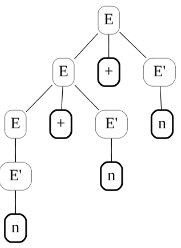
\includegraphics[scale=1]{images/AlberiParsing/associativitaSinistra.png}
      \caption{Associatività Sinistra}
  \end{subfigure}
  \hfill
  \begin{subfigure}{0.45\textwidth}
      \centering
      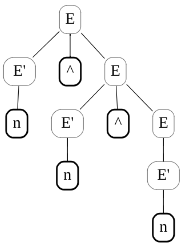
\includegraphics[scale=1]{images/AlberiParsing/associativitiaDestra.png}
      \caption{Associatività Destra}
  \end{subfigure}
  \caption{Confronto tra associatività sinistra e destra}
\end{figure}
 
Quando ho la menata della precedenza, operatori binari con precedenza diversa, questo si trdauce con l'introduzione di simboli ulteriori abbamo or n. Questi simboli sono terminali che rappresentano la precedenza degli operatori.

\begin{lstlisting}
  G_p = Grammar.from_string("""
  E -> E + P | P
  P -> P * F | F
  F -> n
  """)
\end{lstlisting}

\begin{figure}[ht!]
  \centering
  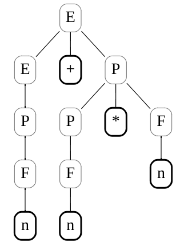
\includegraphics[scale=1]{images/AlberiParsing/precedenza.png}
\end{figure}

Nel caso del dangling else (if else if) diventa una cosa ancora più dolorosa c'è un interplate tra SMUC che è difficile da ricordare risolve la cosa perchè tiene l'else legato all'if più vicino.

\begin{lstlisting}
  G_if = Grammar.from_string("""
  S -> M | U
  M -> if C then M else M | stm
  U -> if C then M else U | if C then S
  C -> cond
  """)
\end{lstlisting}

\begin{figure}[ht!]
  \centering
  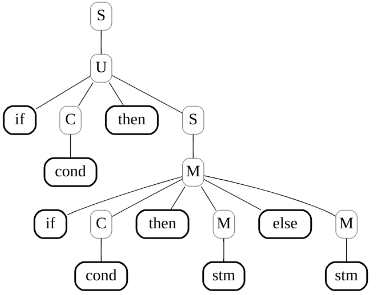
\includegraphics[scale=1]{images/AlberiParsing/dandlingElse.png}
\end{figure}

Il punto cruciale è che context free siamo al giusto livello (non ci siamo persi le parentesi sotto) abbiamo alberi di parsing lineari nella lunghezza della parola, ma dobbiamo stare attenti che avremo ambiguità ed in questo caso dobbiamo o modificare la grammatica che però sarà piena di non terminali e spesso questa procedura passa da trucchi e non c'è niente di teorico (che si possono copiare o inventare).

\end{document}